\chapter{Fotoquímica}\label{ch:b3:photochemistry}

La visión empieza cuando un fotón dobla una molécula. En los bastones del ojo,
el retinal está alojado en su proteína en la forma 11-cis; un fotón de luz verde lo
convierte en la forma todo-trans, y la isomerización se completa prácticamente
en \qty{200}{fs}, más deprisa que casi cualquier otro suceso químico. El resto de la
visión, una enorme amplificación bioquímica, se deriva de esa única molécula
doblada. Las mismas reglas (un fotón excita una molécula, que elige después
entre varios destinos) gobiernan los filtros solares, la síntesis de anillos tensionados,
la terapia fotodinámica, el smog de las ciudades y la \omterm{def:b3:photochemistry:chapman}{capa de ozono} que protege
la superficie de la Tierra de la luz ultravioleta.

\begin{recall}
El \cref{ch:b3:electronic-spectroscopy} describió los estados excitados de las
moléculas, el \omterm{def:b3:electronic-spectroscopy:jablonski}{diagrama de Jablonski}, el \omterm{def:b3:electronic-spectroscopy:radiationless}{cruce entre sistemas}, la \omterm{def:b3:electronic-spectroscopy:luminescence}{fluorescencia} y la
\omterm{def:b3:electronic-spectroscopy:luminescence}{fosforescencia}, la extinción y el \omterm{def:b3:electronic-spectroscopy:quantum-yield}{rendimiento cuántico} de un proceso fotofísico.
El volumen del primer año definió los radicales, la homólisis y los isómeros $Z$/$E$; el volumen del
segundo año, las reacciones concertadas, los orbitales frontera y los ciclos catalíticos.
El \cref{ch:b3:complex-kinetics} trató las \omterm{def:b3:complex-kinetics:chain}{reacciones en cadena} y los estados estacionarios.
\end{recall}

\section{La luz como reactivo}

Dos principios antiguos abren la materia: solo la luz absorbida puede provocar un
cambio químico (Grotthuss y Draper), y cada fotón absorbido excita una
molécula (Stark y Einstein).

\begin{definition}[Flujo de fotones, actinómetro químico]\label{def:b3:photochemistry:photon-flux}
El \emph{flujo de fotones}\index{flujo de fotones} de una fuente de luz es el número de
fotones que emite por unidad de tiempo, contado a menudo en moles de fotones (einstein)
por segundo. Un \emph{actinómetro químico}\index{actinometro quimico@actinómetro químico} es una
reacción fotoquímica de \omterm{def:b3:electronic-spectroscopy:quantum-yield}{rendimiento cuántico} conocido con exactitud que se usa para medir un
flujo de fotones.
\end{definition}

\begin{proposition}[Ley de Stark--Einstein]\label{prop:b3:photochemistry:stark-einstein}
A intensidades luminosas ordinarias, cada fotón absorbido excita exactamente una
molécula; los \omterm{def:b3:electronic-spectroscopy:quantum-yield}{rendimientos cuánticos} primarios de todos los procesos que parten del
estado excitado suman 1.
\end{proposition}

\begin{proof}[Demostración parcial]
Que un fotón sea absorbido por una molécula cada vez se admite (la absorción de dos fotones
exige las intensidades de los láseres pulsados). La molécula excitada
desaparece entonces por procesos de primer orden en competencia, de constantes de velocidad $k_i$
(\cref{ch:b3:electronic-spectroscopy}): la fracción que sigue el camino $i$ es $\Phi_i =
k_i/\sum_jk_j$, y $\sum_i\Phi_i = 1$.
\end{proof}

El \omterm{def:b3:electronic-spectroscopy:quantum-yield}{rendimiento cuántico} de una reacción, el número de moléculas transformadas por fotón
absorbido, no tiene por qué respetar este límite: una etapa fotoquímica primaria puede iniciar una
cadena. Una mezcla de \ce{H2} y \ce{Cl2} expuesta a la luz reacciona con \omterm{def:b3:electronic-spectroscopy:quantum-yield}{rendimientos cuánticos}
de $10^4$ y más, pues cada \ce{Cl2} fotolizado inicia una cadena como la de la
reacción hidrógeno--bromo del \cref{ch:b3:complex-kinetics}; un \omterm{def:b3:electronic-spectroscopy:quantum-yield}{rendimiento cuántico}
mayor que 1 es la firma de una cadena.

\begin{proposition}[Velocidad de una reacción fotoquímica]\label{prop:b3:photochemistry:rate}
Una disolución de absorbancia $A$ a la longitud de onda de irradiación, que recibe un \omterm{def:b3:photochemistry:photon-flux}{flujo
de fotones} $I_0$ (einstein por segundo), absorbe $I_{\mathrm{abs}} = I_0(1 - 10^{-A})$; si el
reactivo lo absorbe todo, la reacción transforma $v = \Phi I_{\mathrm{abs}}$ moles por segundo.
\end{proposition}

\begin{proof}
Por la ley de Beer--Lambert, el flujo transmitido es $I_010^{-A}$, de modo que el absorbido
es $I_0(1 - 10^{-A})$; por definición del \omterm{def:b3:electronic-spectroscopy:quantum-yield}{rendimiento cuántico}, reaccionan $\Phi$ moléculas por
fotón absorbido.
\end{proof}

\begin{method}[La velocidad de una fotorreacción a partir de la lámpara]\label{met:b3:photochemistry:photochemical-rate}
\begin{enumerate}
  \item Energía del fotón, $E = hc/\lambda$; \omterm{def:b3:photochemistry:photon-flux}{flujo de fotones}, $I_0 = P/E$ para una potencia $P$ que llega a la
        muestra, o medido con un actinómetro; dividir por $N_A$ para obtener einstein por
        segundo.
  \item Fracción absorbida, $1 - 10^{-A}$, con $A$ a la longitud de onda de irradiación (que
        cambia a medida que se consume el reactivo).
  \item Velocidad $\Phi I_{\mathrm{abs}}$ en mol/s, dividida por el volumen para obtener una velocidad en concentración.
\end{enumerate}
\end{method}

\begin{method}[Actinometría con ferrioxalato]\label{met:b3:photochemistry:actinometry}
\begin{enumerate}
  \item Irradiar, en la misma celda y la misma geometría que el experimento, una disolución
        acidificada de tris(oxalato)ferrato(III) de potasio, lo bastante concentrada para
        absorber prácticamente toda la luz por debajo de unos \qty{450}{nm}.
  \item La luz reduce el Fe(III) a Fe(II) con un \omterm{def:b3:electronic-spectroscopy:quantum-yield}{rendimiento cuántico} calibrado; tras un
        tiempo medido, añadir 1,10-fenantrolina y tampón, y medir la
        absorbancia del complejo rojo $\ce{[Fe(phen)3]^{2+}}$.
  \item Los moles de Fe(II) divididos por (\omterm{def:b3:electronic-spectroscopy:quantum-yield}{rendimiento cuántico} $\times$ tiempo) dan el \omterm{def:b3:photochemistry:photon-flux}{flujo de fotones}.
\end{enumerate}
\end{method}

\section{Reacciones fotoquímicas}

\begin{definition}[Fotoisomerización, estado fotoestacionario]\label{def:b3:photochemistry:photoisomerisation}
Una \emph{fotoisomerización}\index{fotoisomerizacion@fotoisomerización} es la conversión inducida por la luz
de un isómero en otro, típicamente $E \to Z$ en torno a un doble enlace. Bajo
irradiación continua, dos isómeros que absorben ambos alcanzan un
\emph{estado fotoestacionario}\index{estado fotoestacionario}, una composición estacionaria
fijada por la luz y no por la termodinámica.
\end{definition}

La torsión de un doble enlace explica por qué la luz isomeriza los alquenos. En el
estado fundamental, la energía sube a medida que giran los dos extremos, hasta un máximo a $90^\circ$,
donde el enlace $\pi$ está roto. En el estado excitado $\pi\pi^*$ el orden se invierte: la
geometría girada es la más estable. Una molécula excitada gira hacia
$90^\circ$, donde las dos superficies se juntan, vuelve allí al estado fundamental
y cae hacia uno u otro lado: hacia el isómero del que partió o hacia el
otro.

\begin{omfigure}
\begin{tikzpicture}[font=\small, >=Stealth, x=0.032cm, y=1.1cm]
  \draw[->] (0,0) -- (195,0);
  \node[anchor=north] at (135,-0.45) {ángulo de torsión};
  \draw[->] (0,0) -- (0,5.2) node[anchor=south] {energía};
  \foreach \t/\l in {0/{0^\circ}, 90/{90^\circ}, 180/{180^\circ}}{
    \draw (\t,0) -- (\t,-0.08) node[anchor=north] {$\l$};}
  \draw[thick, black, domain=0:180, samples=90] plot (\x,{2.6*sin(\x)^2 + 0.15*(1-cos(\x))/2});
  \draw[thick, omThm, domain=0:180, samples=90] plot (\x,{4.5 - 1.6*sin(\x)^2 + 0.1*(1-cos(\x))/2});
  \node[anchor=east] at (0,0.15) {$E$};
  \node[anchor=west] at (182,0.2) {$Z$};
  \node[omThm, anchor=south west] at (5,4.55) {$\mathrm S_1$ ($\pi\pi^*$)};
  \node[anchor=north west] at (52,1.2) {$\mathrm S_0$};
  \draw[->, omDef, thick] (12,0.12) -- (12,4.4) node[midway, left] {$h\nu$};
  \draw[->, omDef, thick, decorate, decoration={snake, amplitude=0.6mm, segment length=3mm}] (16,4.4) -- (80,3.05);
  \draw[->, omDef, thick] (90,2.85) -- (90,2.75);
  \draw[->, black!60, thick, domain=96:168, samples=40] plot (\x,{2.6*sin(\x)^2 + 0.15*(1-cos(\x))/2 + 0.28});
  \draw[->, black!60, thick, domain=84:12, samples=40] plot (\x,{2.6*sin(\x)^2 + 0.15*(1-cos(\x))/2 + 0.28});
  \node[font=\scriptsize, anchor=south, align=center] at (90,3.05) {embudo};
\end{tikzpicture}

{\small Estado fundamental ($\mathrm S_0$) y primer estado excitado ($\mathrm S_1$) de un alqueno en función de la
torsión de su doble enlace (esquema). La excitación del isómero $E$ (flecha vertical)
va seguida de la torsión sobre $\mathrm S_1$ hasta la geometría perpendicular, donde las dos
superficies casi se tocan; la molécula vuelve allí a $\mathrm S_0$ y se relaja hacia $E$ o hacia
$Z$.}
\end{omfigure}

\begin{proposition}[Composición fotoestacionaria]\label{prop:b3:photochemistry:pss}
Bajo irradiación monocromática de una disolución ópticamente fina, dos isómeros $E$
y $Z$ de coeficientes de absorción $\varepsilon_E$, $\varepsilon_Z$ y \omterm{def:b3:electronic-spectroscopy:quantum-yield}{rendimientos cuánticos} $\Phi_{E\to Z}$,
$\Phi_{Z\to E}$ alcanzan la razón fotoestacionaria
\[
  \frac{[Z]}{[E]} = \frac{\varepsilon_E\Phi_{E\to Z}}{\varepsilon_Z\Phi_{Z\to E}} .
\]
\end{proposition}

\begin{proof}
En una muestra ópticamente fina, cada isómero absorbe un flujo proporcional a $\varepsilon[\cdot]$, de modo que
$\dd[Z]/\dd t = c(\varepsilon_E\Phi_{E\to Z}[E] - \varepsilon_Z\Phi_{Z\to E}[Z])$, con una constante $c$ fijada por la luz;
el estado estacionario anula el corchete. (El resultado también es válido para muestras
gruesas, pues ambos isómeros se reparten entonces la luz absorbida en la misma proporción.)
\end{proof}

\begin{omfigure}
\begin{tikzpicture}
\begin{axis}[width=0.7\linewidth, height=5.0cm, xmin=0, xmax=120, ymin=0, ymax=1,
  axis lines=left, xlabel={tiempo de irradiación / s}, ylabel={fracción de $Z$},
  tick label style={font=\small}, label style={font=\small}]
\addplot[omDef, very thick] table[x=t, y=Z] {figdata/out/bachelor-3-photostationary.dat};
\draw[black!35, densely dotted] (axis cs:0,0.801) -- (axis cs:60,0.801);
\draw[black!35, densely dotted] (axis cs:60,0.161) -- (axis cs:120,0.161);
\draw[black!35] (axis cs:60,0) -- (axis cs:60,1);
\node[font=\scriptsize, anchor=north] at (axis cs:30,0.98) {\qty{365}{nm}};
\node[font=\scriptsize, anchor=north] at (axis cs:90,0.98) {\qty{440}{nm}};
\node[font=\scriptsize, anchor=south east] at (axis cs:58,0.81) {EFE 0.80};
\node[font=\scriptsize, anchor=south east] at (axis cs:118,0.17) {EFE 0.16};
\end{axis}
\end{tikzpicture}

{\small Un fotointerruptor modelo (una molécula del tipo del azobenceno) irradiado a \qty{365}{nm}, donde
el isómero $E$ absorbe mucho más, y después a \qty{440}{nm}, donde absorbe más el isómero $Z$:
la composición alterna entre dos \omterm{def:b3:photochemistry:photoisomerisation}{estados fotoestacionarios} (EFE; coeficientes de
absorción y \omterm{def:b3:electronic-spectroscopy:quantum-yield}{rendimientos cuánticos} modelo).}
\end{omfigure}

La isomerización 11-cis a todo-trans del retinal en la rodopsina es una
reacción de este tipo, que la proteína hace excepcionalmente rápida y selectiva. Los
fotointerruptores sintéticos basados en el azobenceno o el estilbeno se usan para controlar máquinas
moleculares, materiales y, unidos a fármacos o a canales iónicos, la actividad
biológica mediante la luz.

\begin{definition}[Fotólisis]\label{def:b3:photochemistry:photolysis}
La \emph{fotólisis}\index{fotolisis@fotólisis} es la ruptura de un enlace por la luz. En la
atmósfera, la constante de velocidad de primer orden $j$ de la fotólisis de una especie, su
\emph{constante de velocidad de fotólisis}\index{constante de velocidad de fotolisis@constante de velocidad de fotólisis}, suma sobre
las longitudes de onda el \omterm{def:b3:photochemistry:photon-flux}{flujo de fotones} solar por la sección eficaz de absorción por el
\omterm{def:b3:electronic-spectroscopy:quantum-yield}{rendimiento cuántico}.
\end{definition}

Un fotón solo rompe un enlace si su energía supera la energía de disociación:
$\lambda < hcN_A/D_0$. Para \ce{O2}, $D_0 = 2\Delta_fH^\circ_0(\ce{O}) = \qty{493.6}{kJ/mol}$ según las tablas
termoquímicas, y solo la luz de longitud de onda inferior a \qty{242}{nm} puede romperlo.

Las cetonas y los alquenos excitados también forman enlaces. Dos alquenos, uno de ellos excitado,
se combinan en un ciclobutano: es la fotocicloadición $[2+2]$, prohibida en el
estado fundamental y permitida en el estado excitado por razones orbitales que se dan en el
\cref{ch:b3:pericyclic}. Forma en una sola etapa anillos de cuatro miembros, tensionados y difíciles
de obtener por otras vías.

\begin{definition}[Reacciones de Norrish]\label{def:b3:photochemistry:norrish}
Una \emph{reacción de Norrish de tipo I}\index{reaccion de Norrish de tipo I@reacción de Norrish de tipo I} es la ruptura, por
una cetona excitada, del enlace entre el carbono carbonílico y un carbono $\alpha$,
en un radical acilo y un radical alquilo. Una \emph{reacción de Norrish de tipo
II}\index{reaccion de Norrish de tipo II@reacción de Norrish de tipo II} es la abstracción, por el oxígeno de una
cetona excitada, de un átomo de hidrógeno del carbono $\gamma$, que da un 1,4-birradical
que o bien se rompe en un enol y un alqueno o bien se cierra en un ciclobutanol.
\end{definition}

\begin{omfigure}
\setchemfig{atom sep=1.9em}
\schemestart
\chemfig{H_3C-[:30]C(=[:90]O)-[:-30]CH_2-[:30]CH_2-[:-30]CH_2-[:30]CH_3}
\arrow{->[$h\nu$][vía $\mathrm T_1$]}
\chemfig{H_3C-[:30]\chembelow{C}{\scriptstyle\bullet}(-[:90]OH)-[:-30]CH_2-[:30]CH_2-[:-30]\chemabove{C}{\scriptstyle\bullet}H-[:30]CH_3}
\schemestop

\medskip
\schemestart
\arrow{->[ruptura]}[,1.1]
\chemfig{H_3C-[:30]C(-[:90]OH)=[:-30]CH_2}
\+
\chemfig{H_2C=[:30]CH-[:-30]CH_3}
\schemestop
\hspace{2.5em}
\schemestart
\arrow{->[cierre][del anillo]}[,1.1]
\chemfig{*4(-(-[::-40]OH)(-[::40]CH_3)-(-CH_3)---)}
\schemestop
\par\medskip

{\small La \omterm{def:b3:photochemistry:norrish}{reacción de Norrish de tipo II} de la hexan-2-ona. La cetona triplete abstrae
un hidrógeno del carbono $\gamma$ a través de una disposición de seis miembros; el 1,4-birradical
se rompe en el enol de la acetona (que tautomeriza a acetona) y propeno,
o se cierra en 1,2-dimetilciclobutan-1-ol.}
\end{omfigure}

La fotorreducción de la benzofenona es la versión bimolecular clásica: su
triplete abstrae un átomo de hidrógeno de un disolvente alcohólico como el propan-2-ol,
y dos de los radicales difenilhidroximetilo resultantes se acoplan en benzopinacol,
que cristaliza en la disolución.

\section{Fotosensibilización}

\begin{definition}[Fotosensibilización, oxígeno singlete]\label{def:b3:photochemistry:sensitisation}
Un \emph{fotosensibilizador}\index{fotosensibilizador} es una molécula que absorbe luz
y transfiere la energía o un electrón a otra molécula, que por sí misma no
absorbe: es la \emph{fotosensibilización}\index{fotosensibilizacion@fotosensibilización}. En la
\emph{transferencia de energía triplete}\index{transferencia de energia triplete@transferencia de energía triplete}, el \omterm{def:b3:many-electron-atoms:singlet-triplet}{estado triplete} del
sensibilizador, formado por \omterm{def:b3:electronic-spectroscopy:radiationless}{cruce entre sistemas}, cede su energía al
aceptor por contacto y deja al aceptor en su \omterm{def:b3:many-electron-atoms:singlet-triplet}{estado triplete}. El \emph{oxígeno
singlete}\index{oxigeno singlete@oxígeno singlete} es el estado excitado más bajo de \ce{O2},
${}^1\Delta_g$, que se forma de este modo a partir del oxígeno en su estado fundamental ${}^3\Sigma_g^-$.
\end{definition}

\begin{proposition}[Condición energética de la transferencia triplete]\label{prop:b3:photochemistry:sensitisation-condition}
La transferencia de energía triplete--triplete de un dador D a un aceptor A está próxima al
límite de difusión cuando $E_{\mathrm T}(\mathrm D)$ supera a $E_{\mathrm T}(\mathrm A)$ en más de unos \qty{10}{kJ/mol}, y
cae bruscamente cuando la diferencia se hace negativa.
\end{proposition}

\begin{proof}[Demostración parcial]
La transferencia ${}^3\mathrm D + \mathrm A \to \mathrm D + {}^3\mathrm A$ conserva el espín (dos tripletes cambiados por un
singlete y un triplete) y exige contacto orbital (un mecanismo de intercambio, que se
admite). Su constante de equilibrio es $\exp[(E_{\mathrm T}(\mathrm D) - E_{\mathrm T}(\mathrm A))/RT]$, de unos 60 para un
exceso de \qty{10}{kJ/mol} a \qty{298}{K}: la etapa directa se produce entonces en casi cada
encuentro. Cuando la diferencia es negativa, la constante de velocidad directa es el
límite de difusión multiplicado por el inverso de ese factor (el sentido cuesta arriba paga
el factor de Boltzmann); la curva cuantitativa se admite.
\end{proof}

Un buen sensibilizador absorbe donde el aceptor no lo hace, pasa a su triplete
con un rendimiento alto y tiene un tiempo de vida de triplete largo: la benzofenona, con un
rendimiento de triplete próximo a 1, es la referencia. El \omterm{def:b3:photochemistry:sensitisation}{oxígeno singlete} es un electrófilo
reactivo: se adiciona a los dienos y a los alquenos ricos en electrones. En la terapia
fotodinámica, un sensibilizador que se acumula en un tumor, iluminado a través de una
fibra óptica, produce \omterm{def:b3:photochemistry:sensitisation}{oxígeno singlete} que destruye las células que lo rodean.

\begin{definition}[Catálisis fotorredox]\label{def:b3:photochemistry:photoredox}
La \emph{catálisis fotorredox}\index{catalisis fotorredox@catálisis fotorredox} usa un \omterm{def:b3:photochemistry:sensitisation}{fotosensibilizador}
cuyo estado excitado es a la vez mejor oxidante y mejor reductor que su
estado fundamental para transferir electrones individuales a los sustratos o desde ellos, generando
radicales bajo luz visible; el sensibilizador se regenera en un ciclo
catalítico.
\end{definition}

El complejo de rutenio $\ce{[Ru(bpy)3]^{2+}}$ es el prototipo: su estado excitado de transferencia de
carga del metal al ligando, alcanzado con luz azul y que vive alrededor de un
microsegundo, puede tomar un electrón de una amina o cederlo a un haluro
orgánico. Los radicales formados participan en reacciones de formación de enlaces en
condiciones mucho más suaves que las de la química radicalaria clásica.

\section{Fotoquímica de la atmósfera}

\begin{definition}[Mecanismo de Chapman, capa de ozono]\label{def:b3:photochemistry:chapman}
El \emph{mecanismo de Chapman}\index{mecanismo de Chapman} es el conjunto de las cuatro etapas
\[
  \ce{O2 ->[h\nu] 2 O}\ (j_1), \quad \mathrm{O + O_2 + M \to O_3 + M}\ (k_2), \quad
  \ce{O3 ->[h\nu] O2 + O}\ (j_3), \quad \ce{O + O3 -> 2 O2}\ (k_4).
\]
La \emph{capa de ozono}\index{capa de ozono} es la región de la estratosfera, entre unos
15 y \qty{35}{km} sobre el suelo, donde estas reacciones mantienen las mayores
concentraciones de ozono.
\end{definition}

\begin{theorem}[Estado estacionario de Chapman]\label{thm:b3:photochemistry:chapman}
En el \omterm{def:b3:photochemistry:chapman}{mecanismo de Chapman}, O y \ce{O3} alcanzan el estado estacionario
\[
  \frac{[\ce{O}]}{[\ce{O3}]} = \frac{j_3}{k_2[\mathrm M][\ce{O2}]}, \qquad
  [\ce{O3}] = [\ce{O2}]\sqrt{\frac{j_1k_2[\mathrm M]}{j_3k_4}} .
\]
\end{theorem}

\begin{proof}
O y \ce{O3} se interconvierten rápidamente mediante las etapas 2 y 3 (segundos), mucho más deprisa
de lo que se forman o se destruyen: igualando el intercambio rápido al equilibrio,
$k_2[\ce{O}][\ce{O2}][\mathrm M] = j_3[\ce{O3}]$, se obtiene la razón. Su suma, el oxígeno impar, se forma en la
etapa 1 (dos O por \ce{O2}) y se destruye en la etapa 4 (dos oxígenos impares por suceso):
$2j_1[\ce{O2}] = 2k_4[\ce{O}][\ce{O3}]$. Sustituyendo $[\ce{O}]$ a partir de la razón se obtiene $[\ce{O3}]^2 = j_1k_2[\mathrm M][\ce{O2}]^2/(j_3k_4)$.
\end{proof}

Con las constantes de velocidad de la base de datos evaluada y velocidades de \omterm{def:b3:photochemistry:photolysis}{fotólisis} típicas
de \qty{30}{km} (datos del problema de fin de semana), el modelo de Chapman da unas
$\num{6e12}$ moléculas de ozono por \unit{cm^3}, unas quince partes por millón. Integrada en
altitud, la atmósfera entera contiene por término medio unas 300 unidades Dobson de ozono:
comprimida a la presión del suelo, una capa de \qty{3}{mm} de espesor. El \omterm{def:b3:photochemistry:chapman}{mecanismo de Chapman}
por sí solo predice más ozono del observado: unos ciclos catalíticos lo destruyen más deprisa.

\begin{definition}[Agotamiento del ozono, especie reservorio]\label{def:b3:photochemistry:ozone-depletion}
El \emph{agotamiento del ozono}\index{agotamiento del ozono} es la disminución de la
columna de ozono estratosférico causada por ciclos catalíticos de radicales (Cl y ClO,
NO y \ce{NO2}, OH y \ce{HO2}). Una \emph{especie reservorio}\index{especie reservorio}
es una molécula estable (HCl, \ce{ClONO2}) que retiene un radical catalítico en forma
inactiva, de la que puede liberarse más tarde.
\end{definition}

\begin{omfigure}
\begin{tikzpicture}[font=\small, >=Stealth]
  \node (cl) at (0,0) {Cl};
  \node (clo) at (3.2,0) {ClO};
  \draw[->, thick, omThm] (cl) to[bend left=40] node[midway, above] {$+\,\ce{O3}$, $-\,\ce{O2}$} (clo);
  \draw[->, thick, omThm] (clo) to[bend left=40] node[midway, below] {$+\,\ce{O}$, $-\,\ce{O2}$} (cl);
  \node[font=\scriptsize, align=center] at (1.6,0) {balance\\ $\ce{O + O3 -> 2 O2}$};
  \draw[->, black!55] (cl) -- (-1.6,-1.2) node[below, font=\scriptsize] {$+\,\ce{CH4} \to$ HCl};
  \draw[->, black!55] (clo) -- (4.8,-1.2) node[below, font=\scriptsize] {$+\,\ce{NO2} \to \ce{ClONO2}$};
  \node (o2) at (8.0,1.3) {\ce{O2}};
  \node (o) at (8.0,-1.1) {O};
  \node (o3) at (11.4,-1.1) {\ce{O3}};
  \draw[->, thick] (o2) -- (o) node[midway, left, font=\scriptsize] {$h\nu$};
  \draw[->, thick] (o.south east) to[bend right=30] node[midway, below, font=\scriptsize] {$+\,\ce{O2}$, M} (o3.south west);
  \draw[->, thick] (o3.north west) to[bend right=30] node[midway, above, font=\scriptsize] {$h\nu$} (o.north east);
  \draw[->, thick, black!55] (o3.north) -- (o2.east) node[midway, above right, font=\scriptsize] {$+\,\ce{O}$};
\end{tikzpicture}

{\small Izquierda: el ciclo catalítico del cloro, que destruye una molécula de ozono y
un átomo de oxígeno en cada vuelta y devuelve el átomo de cloro; las flechas grises llevan
a los reservorios. Derecha: el ciclo de Chapman, en el que \ce{O} y \ce{O3} se intercambian
rápidamente por recombinación y \omterm{def:b3:photochemistry:photolysis}{fotólisis} mientras las etapas lentas forman y destruyen
el oxígeno impar.}
\end{omfigure}

\begin{proposition}[Longitud de cadena del ciclo del cloro]\label{prop:b3:photochemistry:catalytic-destruction}
Si en cada vuelta el átomo de Cl reacciona con \ce{O3} con probabilidad $p_1 =
k[\ce{O3}]/(k[\ce{O3}] + k'[\ce{CH4}])$ y el radical ClO con O con probabilidad $p_2 =
k''[\ce{O}]/(k''[\ce{O}] + k'''[\ce{NO2}])$, el número medio de vueltas antes de que el cloro quede
capturado en un reservorio es $p/(1 - p)$, con $p = p_1p_2$; cada vuelta destruye una
molécula de ozono.
\end{proposition}

\begin{proof}
Cada vuelta se completa con probabilidad $p$, independientemente de las
anteriores: el número $n$ de vueltas completas antes de la captura tiene probabilidad $p^n(1 -
p)$, y $\sum_nnp^n(1 - p) = p/(1 - p)$.
\end{proof}

\begin{omfigure}
\begin{tikzpicture}
\begin{axis}[name=oc, width=0.47\linewidth, height=5.2cm, xmin=0, xmax=120, ymin=0, ymax=6.4,
  axis lines=left, xlabel={tiempo / días}, ylabel={$[\ce{O3}]$ / $10^{12}$ \unit{cm^{-3}}},
  tick label style={font=\small}, label style={font=\small},
  legend style={font=\scriptsize, draw=none, fill=white, fill opacity=0.85, text opacity=1,
  at={(0.97,0.03)}, anchor=south east}, legend cell align=left, title={\small estratosfera}]
\addplot[black, thick] table[x=day, y=noCl] {figdata/out/bachelor-3-ozone-chemistry-chapman.dat};
\addplot[omDef, thick] table[x=day, y=Cl1] {figdata/out/bachelor-3-ozone-chemistry-chapman.dat};
\addplot[omThm, thick] table[x=day, y=Cl3] {figdata/out/bachelor-3-ozone-chemistry-chapman.dat};
\legend{Chapman, $+$ \qty{1e7}{cm^{-3}} ClO$_x$, $+$ \qty{3e7}{cm^{-3}} ClO$_x$}
\end{axis}
\begin{axis}[at={(oc.east)}, anchor=west, xshift=1.5cm, width=0.47\linewidth, height=5.2cm,
  xmin=0, xmax=4, ymin=0, ymax=80, axis lines=left, xlabel={$[\ce{NO2}]/[\ce{NO}]$},
  ylabel={$[\ce{O3}]$ / ppb}, tick label style={font=\small}, label style={font=\small},
  title={\small aire contaminado a mediodía}]
\addplot[omDef, very thick] table[x=ratio, y=O3ppb] {figdata/out/bachelor-3-ozone-chemistry-leighton.dat};
\end{axis}
\end{tikzpicture}

{\small Izquierda: el ozono a una altitud modelo de unos \qty{30}{km} (\qty{230}{K}, constantes de velocidad
evaluadas, velocidades de \omterm{def:b3:photochemistry:photolysis}{fotólisis} del problema de fin de semana), que se acumula desde cero
con el \omterm{def:b3:photochemistry:chapman}{mecanismo de Chapman} y queda más bajo con un ciclo del cloro. Derecha: el
\omterm{def:b3:photochemistry:photoisomerisation}{estado fotoestacionario} de Leighton del aire contaminado a \qty{298}{K}, $[\ce{O3}] = j[\ce{NO2}]/k[\ce{NO}]$ con
$j = \qty{8e-3}{s^{-1}}$ (valor modelo a mediodía).}
\end{omfigure}

Cada átomo de cloro, liberado en la estratosfera a partir de los clorofluorocarbonos por
\omterm{def:b3:photochemistry:photolysis}{fotólisis} ultravioleta, destruye ozono durante decenas de vueltas antes de quedar almacenado como
HCl o \ce{ClONO2}, y vuelve a liberarse muchas veces a lo largo de los años que pasa
allí. Sobre la Antártida, en la noche polar, se forman nubes de hielo y de hidrato de ácido
nítrico; en su superficie, los dos reservorios reaccionan entre sí,
$\ce{HCl + ClONO2 -> Cl2 + HNO3}$, el ácido nítrico queda en las partículas y, cuando el
Sol vuelve en primavera, el \ce{Cl2} se fotoliza: sin \ce{NO2}, el cloro no vuelve a
capturarse, y un ciclo a través del dímero de ClO destruye ozono sin
necesitar átomos de O. La columna de ozono cae a unas 100 unidades Dobson: el agujero
de ozono.

\begin{proposition}[Relación de Leighton]\label{prop:b3:photochemistry:leighton}
En un aire iluminado por el Sol en el que el ozono solo se forma por \omterm{def:b3:photochemistry:photolysis}{fotólisis} del \ce{NO2} y solo se destruye
por el NO, las tres especies alcanzan el \omterm{def:b3:photochemistry:photoisomerisation}{estado fotoestacionario}
\[
  [\ce{O3}] = \frac{j_{\ce{NO2}}[\ce{NO2}]}{k[\ce{NO}]} .
\]
\end{proposition}

\begin{proof}
$\ce{NO2 ->[h\nu] NO + O}$ ($j_{\ce{NO2}}$), $\mathrm{O + O_2 + M \to O_3 + M}$ (rápida: cada átomo de O forma un \ce{O3}), y
$\ce{NO + O3 -> NO2 + O2}$ ($k$): en el estado estacionario, el ozono formado, $j_{\ce{NO2}}[\ce{NO2}]$, es igual al
ozono destruido, $k[\ce{NO}][\ce{O3}]$.
\end{proof}

El ciclo por sí solo no forma ozono neto: solo intercambia NO, \ce{NO2} y \ce{O3}. Lo que
aumenta la razón $[\ce{NO2}]/[\ce{NO}]$, y con ella el ozono, es la oxidación de NO a \ce{NO2}
sin consumo de ozono, por radicales peroxilo procedentes de la oxidación de los
hidrocarburos por OH, el detergente de la troposfera.

\begin{definition}[Smog fotoquímico]\label{def:b3:photochemistry:smog}
El \emph{smog fotoquímico}\index{smog fotoquimico@smog fotoquímico} es la mezcla de ozono,
dióxido de nitrógeno, aldehídos, nitratos de peroxiacilo y partículas finas que se forma en el
aire iluminado por el Sol y contaminado por óxidos de nitrógeno y compuestos orgánicos volátiles.
\end{definition}

\begin{omfigure}
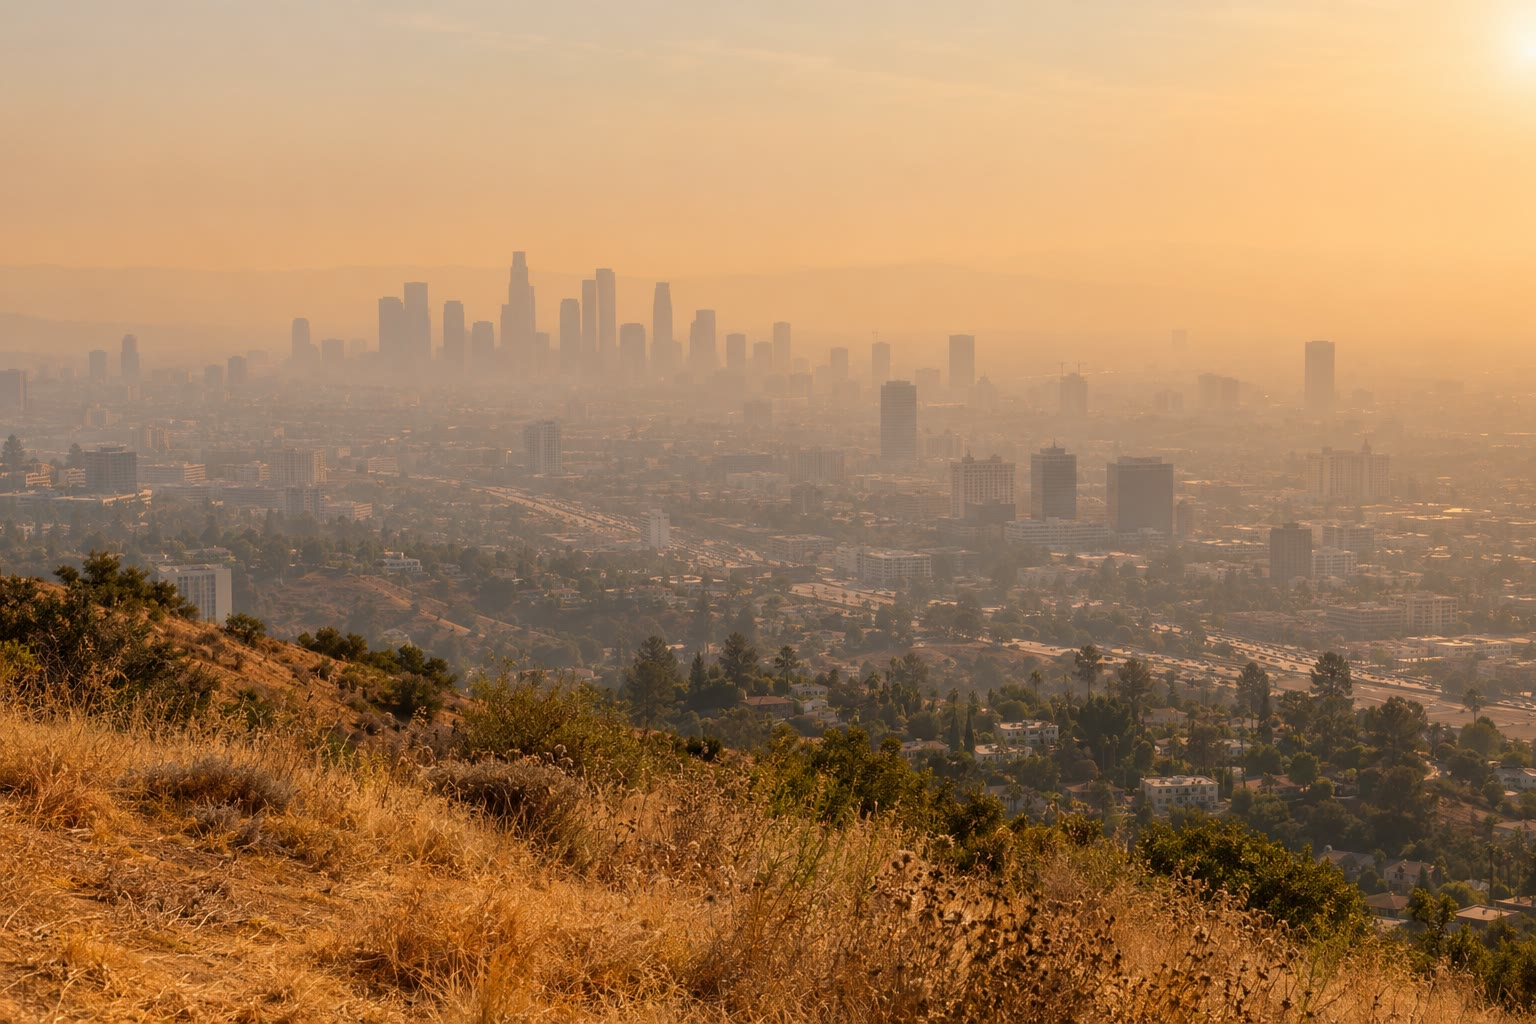
\includegraphics[width=0.6\linewidth]{images/book4/ai/b3-14-smog.jpg}

{\small Una ciudad bajo el \omterm{def:b3:photochemistry:smog}{smog fotoquímico} en una tarde calurosa. El tono pardo procede
del \ce{NO2}; el ozono, que irrita los pulmones, es invisible.}
\end{omfigure}

\begin{omfigure}
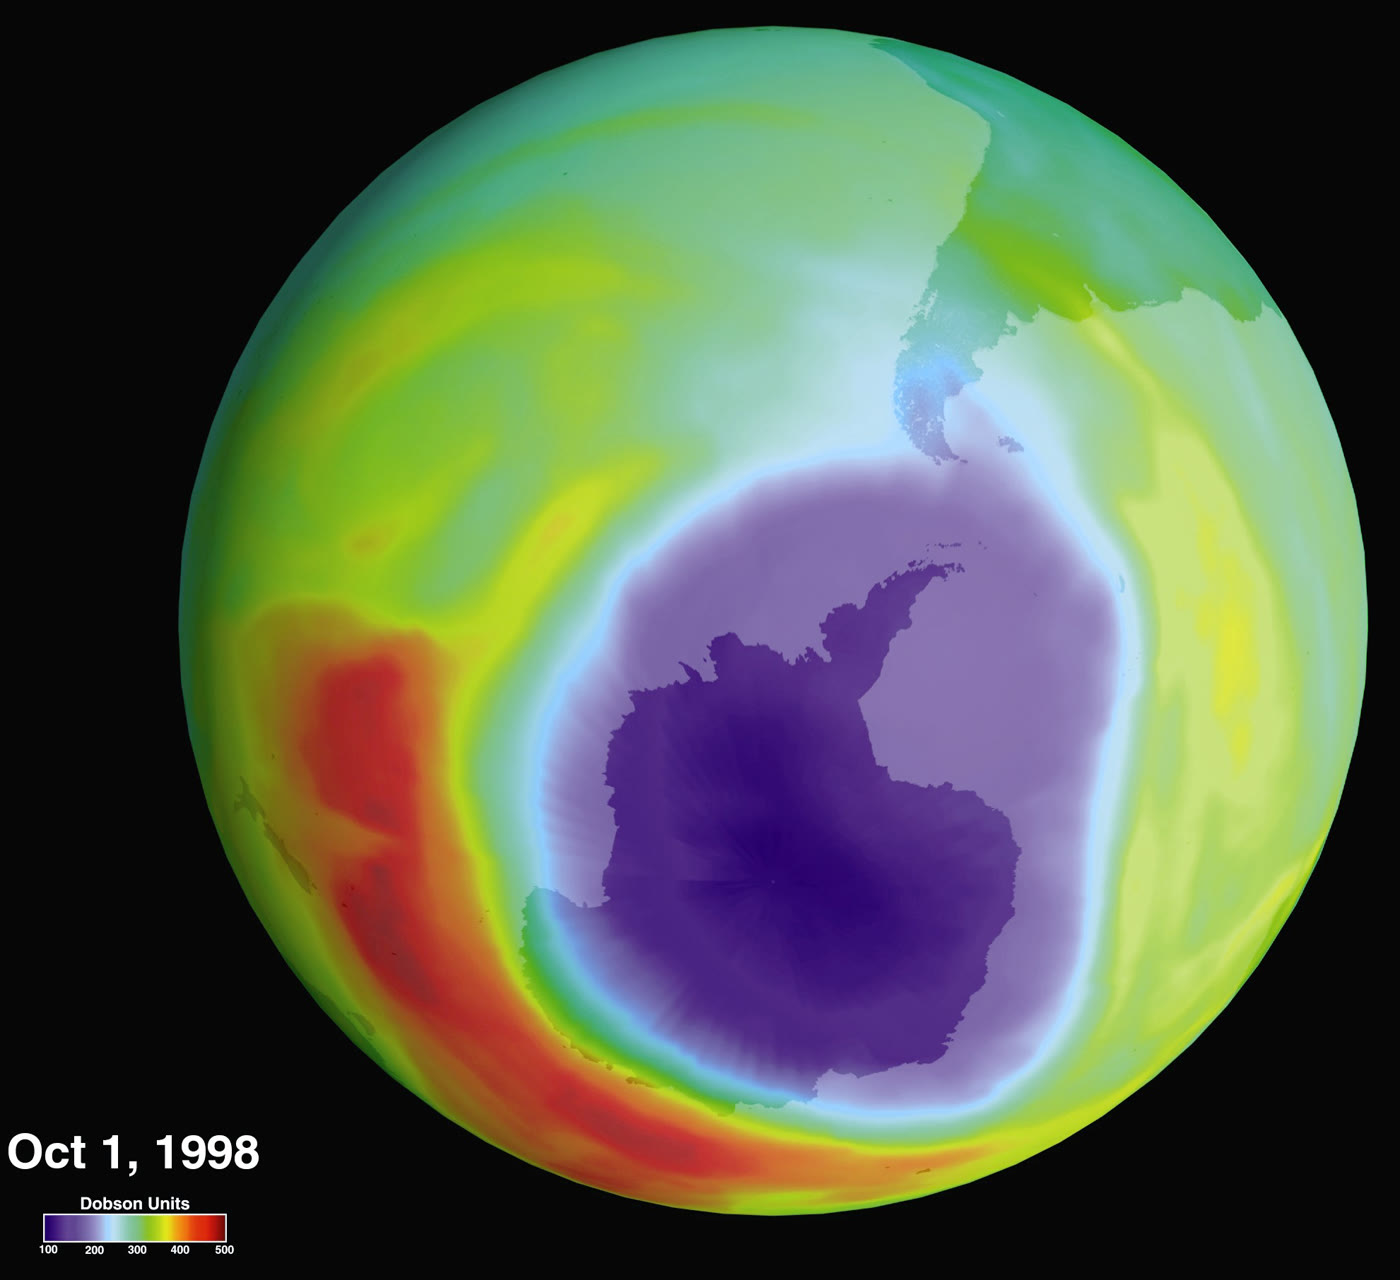
\includegraphics[width=0.5\linewidth]{images/book4/ozone-hole.jpg}

{\small La columna de ozono sobre el hemisferio sur el 1 de octubre de 1998, según
medidas de satélite: el agujero de ozono sobre la Antártida (en morado) cae a unas
100 unidades Dobson, frente a unas 300 en el resto.}
\end{omfigure}

\begin{inthelab}[Un fotorreactor]
Una lámpara de mercurio de media presión, refrigerada en una camisa de cuarzo, ocupa el centro
del recipiente de reacción; una camisa filtrante de vidrio elimina las longitudes de onda por debajo de
unos \qty{300}{nm}, que destruirían los productos. La disolución se
desoxigena con una corriente de nitrógeno (el oxígeno desactiva los tripletes) y se agita.
Todo el reactor está cerrado: la lámpara emite luz ultravioleta dañina para los ojos
y la piel, y nunca se mira directamente, ni siquiera un instante.
\end{inthelab}

\begin{safety}{\ghs[0.8cm]{GHS08}\ghs[0.8cm]{GHS09}}
% ledger: ghs4:benzophenone
Benzofenona, un sensibilizador común y el reactivo de la fotorreducción:
se sospecha que provoca cáncer, puede dañar órganos tras una exposición prolongada y es
tóxica para los organismos acuáticos. Se pesa y se manipula con guantes; los residuos van a los
residuos orgánicos.
\end{safety}

\begin{history}[La fotoquímica del futuro, y el agujero en el cielo]
En 1912, Giacomo Ciamician, en Bolonia, se preguntó si la industria podría funcionar algún día
con la luz del sol, como las plantas, en lugar de con carbón; había pasado años exponiendo
matraces de compuestos orgánicos al sol en la azotea de su laboratorio. En 1985,
tres científicos que trabajaban en una estación de investigación antártica comunicaron que la
columna de ozono primaveral sobre ella venía cayendo bruscamente desde finales de la
década de 1970.
El agujero de ozono, explicado en pocos años por la química de este capítulo,
condujo a la eliminación progresiva de los clorofluorocarbonos.
\end{history}

\section{Ejercicios}

\begin{exercise}[$\star$]\label{exo:b3:photochemistry:1}
Una lámpara entrega \qty{100}{mW} a \qty{365}{nm}. ¿Cuántos fotones por segundo, y cuántos
einstein por segundo?
\end{exercise}

\begin{exercise}[$\star$]\label{exo:b3:photochemistry:2}
En \qty{10.0}{min}, una disolución que absorbe \qty{1.00e-7}{einstein.s^{-1}} transforma
\qty{2.0e-5}{mol} de reactivo. Calcúlese el \omterm{def:b3:electronic-spectroscopy:quantum-yield}{rendimiento cuántico}.
\end{exercise}

\begin{exercise}[$\star$]\label{exo:b3:photochemistry:3}
La reacción fotoquímica de \ce{H2} con \ce{Cl2} tiene \omterm{def:b3:electronic-spectroscopy:quantum-yield}{rendimientos cuánticos} de hasta $10^4$ y
más. ¿Qué muestra esto? Escríbanse las etapas de propagación.
\end{exercise}

\begin{exercise}[$\star$]\label{exo:b3:photochemistry:4}
% ledger: janaf:O.dfH0, janaf:O3.dfH0
A partir de las entalpías de formación a 0 K de O (\qty{246.79}{kJ/mol}) y de \ce{O3}
(\qty{145.35}{kJ/mol}), calcúlense las longitudes de onda máximas capaces de romper \ce{O2} en dos
átomos y \ce{O3} en \ce{O2} y O.
\end{exercise}

\begin{exercise}[$\star\star$]\label{exo:b3:photochemistry:5}
Un fotointerruptor tiene, a \qty{365}{nm}, $\varepsilon_E = 22\,000$ y $\varepsilon_Z = 1500$ \unit{L.mol^{-1}.cm^{-1}}, con
$\Phi_{E\to Z} = 0.11$ y $\Phi_{Z\to E} = 0.40$ (datos del ejercicio). Calcúlese la composición
fotoestacionaria.
\end{exercise}

\begin{exercise}[$\star\star$]\label{exo:b3:photochemistry:6}
Dense los productos de la \omterm{def:b3:photochemistry:norrish}{reacción de Norrish de tipo II} de la hexan-2-ona, y explíquese
por qué la pentan-2-ona da eteno en lugar de propeno.
\end{exercise}

\begin{exercise}[$\star\star$]\label{exo:b3:photochemistry:7}
Un aceptor tiene una energía de triplete de \qty{250}{kJ/mol}. De tres
sensibilizadores candidatos con energías de triplete de 289, 253 y \qty{236}{kJ/mol} (datos del
ejercicio), ¿cuál transfiere eficazmente? Estímese la constante de equilibrio de la
transferencia para cada uno a \qty{298}{K}.
\end{exercise}

\begin{exercise}[$\star\star$]\label{exo:b3:photochemistry:8}
% ledger: kin:O+O2+M.k0, kin:O+O2+M.n
A \qty{230}{K}, con $[\mathrm M] = \qty{4.0e17}{cm^{-3}}$, $[\ce{O2}] = 0.21[\mathrm M]$ y $j_3 = \qty{1.0e-3}{s^{-1}}$,
calcúlense $k_2$ y la razón estacionaria $[\ce{O}]/[\ce{O3}]$.
\end{exercise}

\begin{exercise}[$\star\star$]\label{exo:b3:photochemistry:9}
% ledger: kin:Cl+O3.A, kin:Cl+O3.EaR, kin:Cl+CH4.A, kin:Cl+CH4.EaR
A \qty{230}{K}, calcúlense las constantes de velocidad de $\ce{Cl + O3}$ y de $\ce{Cl + CH4}$, y la
probabilidad de que un átomo de Cl encuentre \ce{O3} y no \ce{CH4} cuando $[\ce{O3}] = \qty{5.7e12}{cm^{-3}}$
y $[\ce{CH4}] = \qty{4.0e11}{cm^{-3}}$.
\end{exercise}

\begin{exercise}[$\star\star\star$]\label{exo:b3:photochemistry:10}
% ledger: kin:NO+O3.A, kin:NO+O3.EaR
A mediodía en una ciudad, $[\ce{NO2}]/[\ce{NO}] = 1.5$ y $j_{\ce{NO2}} = \qty{8.0e-3}{s^{-1}}$. Calcúlese el
ozono fotoestacionario a \qty{298}{K} en moléculas por \unit{cm^3} y en ppb (aire a \qty{1}{bar}).
¿Qué ocurre de noche?
\end{exercise}

\begin{exercise}[$\star\star\star$]\label{exo:b3:photochemistry:11}
Una disolución de \qty{3.0}{mL} de absorbancia 0.50 a \qty{313}{nm} recibe \qty{50}{mW} de
luz a esa longitud de onda; la reacción tiene $\Phi = 0.25$. Calcúlese la velocidad inicial en
\unit{mol.L^{-1}.s^{-1}}.
\end{exercise}

\begin{exercise}[$\star\star\star$]\label{exo:b3:photochemistry:12}
Un actinómetro de ferrioxalato, con un \omterm{def:b3:electronic-spectroscopy:quantum-yield}{rendimiento cuántico} de 1.25 a \qty{365}{nm} (datos del
ejercicio) y absorción total, forma \qty{3.0e-6}{mol} de Fe(II) en \qty{60}{s}.
Calcúlese el \omterm{def:b3:photochemistry:photon-flux}{flujo de fotones}. ¿Por qué debe mantenerse pequeña la conversión?
\end{exercise}

\section{Problema: hacer y deshacer la capa de ozono}

\begin{problem}[{Problema de fin de semana --- hacer y deshacer la capa de ozono: umbrales
de los fotones, el estado estacionario de Chapman con constantes de velocidad evaluadas, el
ciclo del cloro y los reservorios que lo detienen}]
\label{pb:b3:photochemistry:1}
% ledger: janaf:O.dfH0, janaf:O3.dfH0, kin:O+O2+M.k0, kin:O+O2+M.n, kin:O+O3.A, kin:O+O3.EaR, kin:Cl+O3.A, kin:Cl+O3.EaR, kin:O+ClO.A, kin:O+ClO.EaR, kin:Cl+CH4.A, kin:Cl+CH4.EaR, kin:ClO+NO2+M.k0, kin:ClO+NO2+M.n, kin:ClO+NO2+M.kinf, kin:ClO+NO2+M.Fc, oz:column.mean, oz:column.hole
Un modelo de la estratosfera hacia \qty{30}{km} (datos del problema): $T = \qty{230}{K}$, $[\mathrm M] =
\qty{4.0e17}{cm^{-3}}$, $[\ce{O2}] = 0.21[\mathrm M]$, \omterm{def:b3:photochemistry:photolysis}{constantes de velocidad de fotólisis} $j_1 = \qty{1.0e-11}{s^{-1}}$ (\ce{O2})
y $j_3 = \qty{1.0e-3}{s^{-1}}$ (\ce{O3}), $[\ce{CH4}] = \qty{4.0e11}{cm^{-3}}$, $[\ce{NO2}] = \qty{1.0e9}{cm^{-3}}$. Constantes de velocidad
evaluadas (\unit{cm^3.s^{-1}}, o \unit{cm^6.s^{-1}} para $k_2$, contando las concentraciones por \unit{cm^3}):
$k_2 = \num{6.0e-34}(T/300)^{-2.6}$; $k_4 = \num{8.0e-12}\eu^{-2060/T}$; Cl + \ce{O3}: $\num{2.8e-11}\eu^{-250/T}$;
O + ClO: $\num{2.5e-11}\eu^{110/T}$; Cl + \ce{CH4}: $\num{6.6e-12}\eu^{-1240/T}$; ClO + \ce{NO2} + M: $\num{1.41e-13}$ en
estas condiciones.

\medskip\noindent\textbf{Parte I --- Umbrales de los fotones.}
\begin{enumerate}
  \item Calcúlese $D_0(\ce{O2})$ a partir de $\Delta_fH^\circ_0(\ce{O}) = \qty{246.79}{kJ/mol}$.
  \item Dedúzcase la longitud de onda máxima que rompe \ce{O2}.
  \item Calcúlese la energía de $\ce{O3 -> O2 + O}$ ($\Delta_fH^\circ_0(\ce{O3}) = \qty{145.35}{kJ/mol}$) y su
        longitud de onda umbral.
  \item La luz visible podría, pues, romper el ozono; ¿por qué es la absorción ultravioleta
        del ozono la que importa para la vida?
  \item ¿Por qué el \ce{O2} solo se fotoliza en las capas altas de la atmósfera?
\end{enumerate}

\medskip\noindent\textbf{Parte II --- El estado estacionario de Chapman.}
\begin{enumerate}[resume]
  \item Escríbanse las cuatro etapas de Chapman.
  \item Calcúlense $k_2$ y $k_2[\mathrm M]$ a \qty{230}{K}.
  \item Calcúlese $k_4$.
  \item Calcúlese $[\ce{O}]/[\ce{O3}]$.
  \item Demuéstrese que $[\ce{O3}] = [\ce{O2}]\sqrt{j_1k_2[\mathrm M]/(j_3k_4)}$.
  \item Calcúlense $[\ce{O3}]$ y su fracción molar.
  \item Calcúlese $[\ce{O}]$.
  \item El ozono observado es inferior. ¿Por qué?
\end{enumerate}

\medskip\noindent\textbf{Parte III --- El ciclo del cloro.}
\begin{enumerate}[resume]
  \item Escríbanse el ciclo y su reacción global.
  \item Calcúlese el tiempo de vida de un átomo de Cl frente al \ce{O3}.
  \item Calcúlese el tiempo de vida del ClO frente al O.
  \item Dedúzcase la razón estacionaria $[\ce{ClO}]/[\ce{Cl}]$.
  \item Con $[\ce{Cl}] + [\ce{ClO}] = \qty{1.0e7}{cm^{-3}}$, compárese la velocidad de pérdida de oxígeno impar por el
        ciclo con la de la etapa de Chapman $\ce{O + O3}$.
  \item ¿Qué etapa limita el ciclo?
\end{enumerate}

\medskip\noindent\textbf{Parte IV --- Los reservorios.}
\begin{enumerate}[resume]
  \item Calcúlese la probabilidad de que un átomo de Cl reaccione con \ce{O3} y no con
        \ce{CH4}.
  \item Calcúlese la probabilidad de que el ClO reaccione con O y no con \ce{NO2}.
  \item Dedúzcase la probabilidad $p$ de que se complete una vuelta del ciclo.
  \item Dedúzcase el número medio de vueltas antes de que el cloro quede capturado.
  \item Explíquese cómo alargan la cadena las nubes estratosféricas polares.
  \item Enúnciese el resultado: el número de moléculas de ozono que destruye un átomo de cloro,
        en este modelo, antes de quedar capturado en un reservorio.
\end{enumerate}
\end{problem}
